% Birthday problem: exact, Poisson, Chen-Stein band (generated by a script).
\begin{tikzpicture}[x=1cm,y=1cm]
\fill[blue!12] (0.150,4.000) -- (0.300,3.989) -- (0.450,3.968) -- (0.600,3.936) -- (0.750,3.896) -- (0.900,3.846) -- (1.050,3.789) -- (1.200,3.725) -- (1.350,3.654) -- (1.500,3.578) -- (1.650,3.497) -- (1.800,3.413) -- (1.950,3.325) -- (2.100,3.236) -- (2.250,3.145) -- (2.400,3.054) -- (2.550,2.964) -- (2.700,2.874) -- (2.850,2.787) -- (3.000,2.701) -- (3.150,2.619) -- (3.300,2.541) -- (3.450,2.466) -- (3.600,2.395) -- (3.750,2.330) -- (3.900,2.269) -- (4.050,2.213) -- (4.200,2.162) -- (4.350,2.117) -- (4.500,2.077) -- (4.650,2.042) -- (4.800,2.013) -- (4.950,1.989) -- (5.100,1.970) -- (5.250,1.956) -- (5.400,1.946) -- (5.550,1.941) -- (5.700,1.940) -- (5.850,1.944) -- (6.000,1.951) -- (6.150,1.962) -- (6.300,1.976) -- (6.450,1.993) -- (6.600,2.013) -- (6.750,2.036) -- (6.900,2.061) -- (7.050,2.088) -- (7.200,2.117) -- (7.350,2.148) -- (7.500,2.181) -- (7.650,2.215) -- (7.800,2.250) -- (7.950,2.287) -- (8.100,2.324) -- (8.250,2.363) -- (8.400,2.402) -- (8.550,2.442) -- (8.700,2.482) -- (8.850,2.523) -- (9.000,2.565) -- (9.000,0.000) -- (8.850,0.000) -- (8.700,0.000) -- (8.550,0.000) -- (8.400,0.000) -- (8.250,0.000) -- (8.100,0.000) -- (7.950,0.000) -- (7.800,0.000) -- (7.650,0.000) -- (7.500,0.000) -- (7.350,0.000) -- (7.200,0.000) -- (7.050,0.000) -- (6.900,0.000) -- (6.750,0.000) -- (6.600,0.000) -- (6.450,0.000) -- (6.300,0.000) -- (6.150,0.000) -- (6.000,0.000) -- (5.850,0.000) -- (5.700,0.000) -- (5.550,0.000) -- (5.400,0.000) -- (5.250,0.000) -- (5.100,0.000) -- (4.950,0.000) -- (4.800,0.042) -- (4.650,0.195) -- (4.500,0.352) -- (4.350,0.513) -- (4.200,0.678) -- (4.050,0.845) -- (3.900,1.015) -- (3.750,1.187) -- (3.600,1.360) -- (3.450,1.534) -- (3.300,1.708) -- (3.150,1.881) -- (3.000,2.052) -- (2.850,2.221) -- (2.700,2.386) -- (2.550,2.548) -- (2.400,2.704) -- (2.250,2.855) -- (2.100,2.999) -- (1.950,3.135) -- (1.800,3.264) -- (1.650,3.384) -- (1.500,3.494) -- (1.350,3.594) -- (1.200,3.684) -- (1.050,3.763) -- (0.900,3.831) -- (0.750,3.888) -- (0.600,3.933) -- (0.450,3.967) -- (0.300,3.989) -- (0.150,4.000) -- cycle;
\draw[black!35,->] (0,0)--(9.4,0) node[right,font=\scriptsize,black!60]{$n$};
\draw[black!35,->] (0,0)--(0,4.3);
\draw[black!35] (0.00,0.05)--(0.00,-0.05) node[below,font=\tiny,black!60]{$0$};
\draw[black!35] (1.50,0.05)--(1.50,-0.05) node[below,font=\tiny,black!60]{$10$};
\draw[black!35] (3.00,0.05)--(3.00,-0.05) node[below,font=\tiny,black!60]{$20$};
\draw[black!35] (4.50,0.05)--(4.50,-0.05) node[below,font=\tiny,black!60]{$30$};
\draw[black!35] (6.00,0.05)--(6.00,-0.05) node[below,font=\tiny,black!60]{$40$};
\draw[black!35] (7.50,0.05)--(7.50,-0.05) node[below,font=\tiny,black!60]{$50$};
\draw[black!35] (9.00,0.05)--(9.00,-0.05) node[below,font=\tiny,black!60]{$60$};
\draw[black!35] (0.05,1.00)--(-0.05,1.00) node[left,font=\tiny,black!60]{$0.25$};
\draw[black!35] (0.05,2.00)--(-0.05,2.00) node[left,font=\tiny,black!60]{$0.50$};
\draw[black!35] (0.05,3.00)--(-0.05,3.00) node[left,font=\tiny,black!60]{$0.75$};
\draw[black!35] (0.05,4.00)--(-0.05,4.00) node[left,font=\tiny,black!60]{$1.00$};
\draw[black!25,dashed] (3.45,0)--(3.45,2.00);
\draw[red!70!black,thick] (0.150,4.000) -- (0.300,3.989) -- (0.450,3.967) -- (0.600,3.935) -- (0.750,3.892) -- (0.900,3.839) -- (1.050,3.776) -- (1.200,3.705) -- (1.350,3.624) -- (1.500,3.536) -- (1.650,3.440) -- (1.800,3.338) -- (1.950,3.230) -- (2.100,3.117) -- (2.250,3.000) -- (2.400,2.879) -- (2.550,2.756) -- (2.700,2.630) -- (2.850,2.504) -- (3.000,2.377) -- (3.150,2.250) -- (3.300,2.124) -- (3.450,2.000) -- (3.600,1.878) -- (3.750,1.758) -- (3.900,1.642) -- (4.050,1.529) -- (4.200,1.420) -- (4.350,1.315) -- (4.500,1.215) -- (4.650,1.119) -- (4.800,1.028) -- (4.950,0.941) -- (5.100,0.860) -- (5.250,0.784) -- (5.400,0.712) -- (5.550,0.645) -- (5.700,0.583) -- (5.850,0.525) -- (6.000,0.472) -- (6.150,0.423) -- (6.300,0.378) -- (6.450,0.337) -- (6.600,0.300) -- (6.750,0.266) -- (6.900,0.235) -- (7.050,0.207) -- (7.200,0.182) -- (7.350,0.160) -- (7.500,0.139) -- (7.650,0.122) -- (7.800,0.106) -- (7.950,0.092) -- (8.100,0.079) -- (8.250,0.068) -- (8.400,0.059) -- (8.550,0.050) -- (8.700,0.043) -- (8.850,0.037) -- (9.000,0.031);
\fill[black] (0.150,4.000) circle (0.04);
\fill[black] (0.450,3.967) circle (0.04);
\fill[black] (0.750,3.891) circle (0.04);
\fill[black] (1.050,3.775) circle (0.04);
\fill[black] (1.350,3.622) circle (0.04);
\fill[black] (1.650,3.435) circle (0.04);
\fill[black] (1.950,3.222) circle (0.04);
\fill[black] (2.250,2.988) circle (0.04);
\fill[black] (2.550,2.740) circle (0.04);
\fill[black] (2.850,2.484) circle (0.04);
\fill[black] (3.150,2.225) circle (0.04);
\fill[black] (3.450,1.971) circle (0.04);
\fill[black] (3.750,1.725) circle (0.04);
\fill[black] (4.050,1.493) circle (0.04);
\fill[black] (4.350,1.276) circle (0.04);
\fill[black] (4.650,1.078) circle (0.04);
\fill[black] (4.950,0.900) circle (0.04);
\fill[black] (5.250,0.742) circle (0.04);
\fill[black] (5.550,0.605) circle (0.04);
\fill[black] (5.850,0.487) circle (0.04);
\fill[black] (6.150,0.387) circle (0.04);
\fill[black] (6.450,0.304) circle (0.04);
\fill[black] (6.750,0.236) circle (0.04);
\fill[black] (7.050,0.181) circle (0.04);
\fill[black] (7.350,0.137) circle (0.04);
\fill[black] (7.650,0.102) circle (0.04);
\fill[black] (7.950,0.075) circle (0.04);
\fill[black] (8.250,0.055) circle (0.04);
\fill[black] (8.550,0.040) circle (0.04);
\fill[black] (8.850,0.028) circle (0.04);
\node[font=\scriptsize,anchor=west] at (5.2,3.4) {\textcolor{red!70!black}{$e^{-\binom n2/365}$}};
\node[font=\scriptsize,anchor=west] at (5.2,2.95) {$\bullet$ exact};
\end{tikzpicture}
